\clearpage
\setcounter{page}{1}
\section{Variationsrechnung \label{sec:varrec}}



\subsection{Stab unter Eigengewicht}

\begin{minipage}{0.3\textwidth}
% \centering \raisebox{\dimexpr-\height+1.5ex\relax}{\includegraphics[scale=0.8]{fig/ue2_stab_eigengewicht.pdf}} % workarount if top alignment is needed
\center
\includegraphics[scale=0.8]{fig/ue2_stab_eigengewicht.pdf}
\end{minipage}
\hfill
\begin{minipage}{0.64\textwidth}
Ein Stab ($EA=const.$) der Dichte $\rho$ und der Länge $l$ ist eingespannt an der Position $x=0$ und erfährt eine Deformation aufgrund seiner Masse im Erdschwerefeld $g$.
\enab
\item Leiten Sie mithilfe des Prinzips des Minimums des elastischen Gesamtpotentials die Euler-Lagrange Differentialgleichung für die Verschiebungsfunktion $u(x)$ her.
\item Ermitteln sie die Lösungsfunktion $u(x)$ der Differentialgleichung unter Berücksichtigung der Randbedingungen.
\enae
\end{minipage}





\subsection{Balken unter Streckenlast}

Ein Balken ($EI=const.$) der Länge $l$ erfährt eine konstante Streckenlast $q(x)=q_0$. 

\begin{center}
\includegraphics[width=0.44\textwidth]{fig/ue2_balken_linienlast.pdf}
\end{center}

Vorgegeben sei das folgende elastische Gesamtpotential:
%
\ebn
\Pi=\int_{0}^l \Big[ \frac{1}{2} EI(w(x)'')^2-w(x)q_0 \Big] \intd{x}
\een

\enab
\item Leiten Sie mithilfe der Variationsmethode die Euler-Lagrange Gleichung für die Durchbiegung $w(x)$ sowie die natürlichen Randbedingungen her.
\item Bestimmen sie die Biegelinie $w(x)$ unter Auswertung der Randbedingungen
\item Wie lauten die natürlichen Randbedingungen unter der Annahme, dass der Balken bei $x=0$ fest eingespannt ist und bei $x=l$ frei?
\par \textit{Hinweis}: Die essentiellen RB lauten in diesem Fall $w(0)=0$ und $w'(0)=0$.
\enae



